\documentclass[border=10pt]{standalone}
\usepackage{tikz}
\usepackage{pgfplots}
\pgfplotsset{compat=1.18}
\usetikzlibrary{arrows.meta,decorations.markings,calc}

\begin{document}
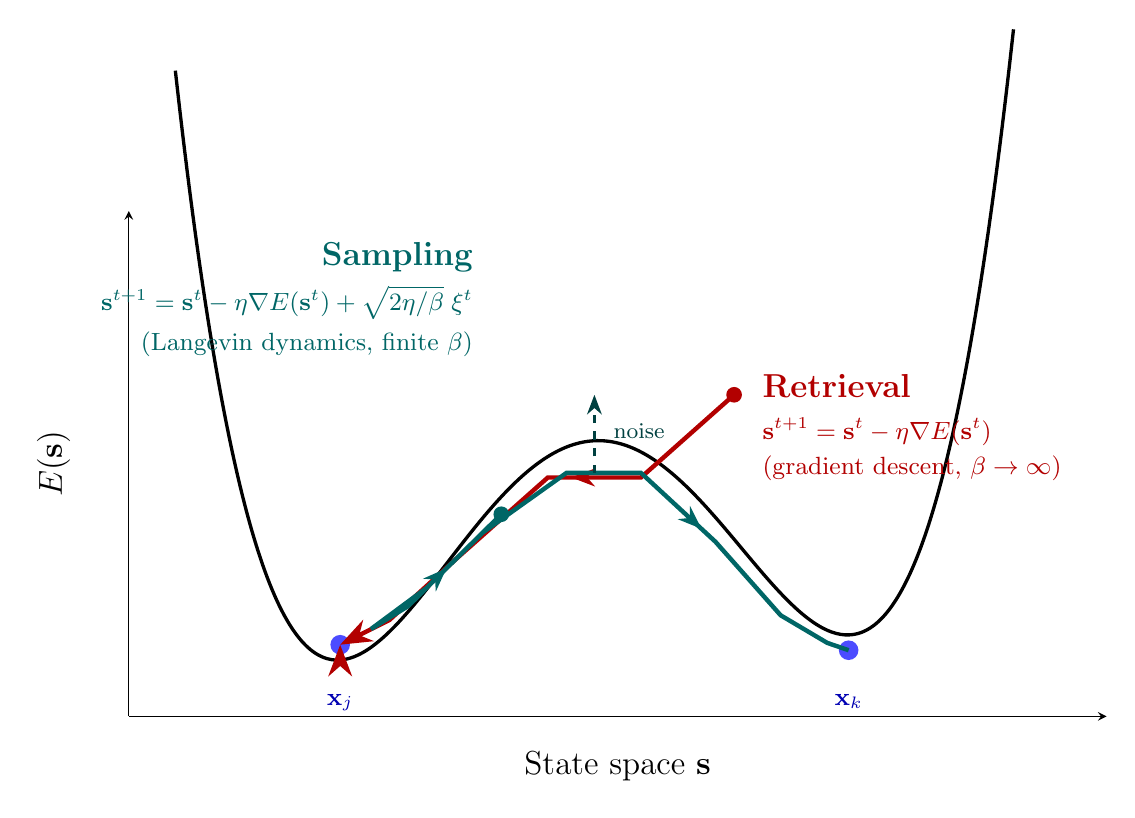
\begin{tikzpicture}

% Energy landscape function (double-well style)
\def\energy#1{0.04*(#1)^4 - 0.6*(#1)^2 + 0.05*(#1) + 2.5}

% Draw energy surface
\begin{axis}[
    width=14cm, height=8cm,
    domain=-4.5:4.5,
    samples=200,
    axis lines=left,
    xlabel={State space $\mathbf{s}$},
    ylabel={$E(\mathbf{s})$},
    xlabel style={font=\large, at={(axis description cs:0.5,-0.05)}},
    ylabel style={font=\large, at={(axis description cs:-0.05,0.5)}},
    xtick=\empty,
    ytick=\empty,
    ymin=-0.5, ymax=5,
    xmin=-5, xmax=5.5,
    clip=false,
    every axis plot/.append style={thick},
]

% Energy curve
\addplot[black, very thick, smooth] {0.04*x^4 - 0.6*x^2 + 0.05*x + 2.5};

% Left minimum marker
\node[circle, fill=blue!70, inner sep=2.5pt] at (axis cs:-2.73,0.28) {};
\node[below, font=\small, blue!70!black] at (axis cs:-2.73,-0.15) {$\mathbf{x}_j$};

% Right minimum marker
\node[circle, fill=blue!70, inner sep=2.5pt] at (axis cs:2.73,0.22) {};
\node[below, font=\small, blue!70!black] at (axis cs:2.73,-0.15) {$\mathbf{x}_k$};

% --- Retrieval trajectory (gradient descent) ---
% Starting point high on left slope
\addplot[red!70!black, ultra thick, -{Stealth[length=4mm]},
    decoration={markings, mark=at position 0.4 with {\arrow{Stealth[length=3mm]}}},
    postaction={decorate}]
    coordinates {(1.5, 3.0) (0.5, 2.1) (-0.5, 2.1) (-1.5, 1.2) (-2.2, 0.55) (-2.73,0.28)};

% Retrieval label
\node[red!70!black, font=\large\bfseries, anchor=west] at (axis cs:1.7, 3.1) {Retrieval};
\node[red!70!black, font=\small, anchor=west] at (axis cs:1.7, 2.6) {$\mathbf{s}^{t+1} = \mathbf{s}^t - \eta\nabla E(\mathbf{s}^t)$};
\node[red!70!black, font=\small, anchor=west] at (axis cs:1.7, 2.2) {(gradient descent, $\beta \to \infty$)};

% --- Sampling trajectory (Langevin) ---
% Wiggly path that explores both wells
\addplot[teal!80!black, ultra thick,
    decoration={markings, mark=at position 0.35 with {\arrow{Stealth[length=3mm]}},
                          mark=at position 0.75 with {\arrow{Stealth[length=3mm]}}},
    postaction={decorate}]
    coordinates {(-1.0, 1.7) (-1.8, 0.9) (-2.4, 0.45) (-2.0, 0.7) (-1.2, 1.5)
                 (-0.3, 2.15) (0.5, 2.15) (1.3, 1.4) (2.0, 0.6) (2.5, 0.3)
                 (2.73, 0.22)};

% Sampling label
\node[teal!80!black, font=\large\bfseries, anchor=east] at (axis cs:-1.2, 4.5) {Sampling};
\node[teal!80!black, font=\small, anchor=east] at (axis cs:-1.2, 4.0) {$\mathbf{s}^{t+1} = \mathbf{s}^t - \eta\nabla E(\mathbf{s}^t) + \sqrt{2\eta/\beta}\;\boldsymbol{\xi}^t$};
\node[teal!80!black, font=\small, anchor=east] at (axis cs:-1.2, 3.55) {(Langevin dynamics, finite $\beta$)};

% Start markers
\node[circle, fill=red!70!black, inner sep=2pt] at (axis cs:1.5, 3.0) {};
\node[circle, fill=teal!80!black, inner sep=2pt] at (axis cs:-1.0, 1.7) {};

% Noise annotation
\draw[teal!50!black, thick, dashed, -{Stealth[length=2.5mm]}]
    (axis cs:0.0, 2.15) -- (axis cs:0.0, 3.0);
\node[teal!50!black, font=\footnotesize, anchor=west] at (axis cs:0.1, 2.6) {noise};

\end{axis}
\end{tikzpicture}
\end{document}
